% Chapter Template

\chapter{Implémentation et évaluation expérimentale} % Main chapter title

\label{Chapter4} % Change X to a consecutive number; for referencing this chapter elsewhere, use \ref{ChapterX}

%----------------------------------------------------------------------------------------
%	SECTION 1
%----------------------------------------------------------------------------------------

\section{Introduction}
Après avoir étudié le domaine de CBIR (les systèmes de recherche d’images par le contenu ) et leur principe de fonctionnement, l’implémentation d’une application ou d’un système de recherche d’images par le contenu devient une nécessité afin d’avoir une vue plus claire de ce que nous avons introduit dans les premiers chapitres. \\

Nous présenterons alors, dans ce chapitre, notre application,
les descripteurs utilisés et les bases d’images choisies afin de pouvoir évaluer le système, ainsi les différentes étapes par lesquelles nous sommes passés pour sa réalisation.

\section{L'outil d’implémentation}
Dans la conception de notre application, nous avons choisi Python
comme langage de programmation, ce choix est justifié par plusieurs
facteurs, parmi eux on cite:
\begin{itemize}
	\item Une librairie très riche, il est complété par de multiples boîtes à outils (le calcul numérique matriciel avec Numpy, vision par ordinateur avec OpenCV, ...etc).
	\item Une syntaxe simple permettant une souplesse durant l'implémentation.
	\item Possible d’exécuter le code en dehors du programme (Testes unitaires).
	\item Une aide très bien faite.
	\item Opensource contrairement à Matlab.
\end{itemize}

\begin{figure}[H]
	\centering
	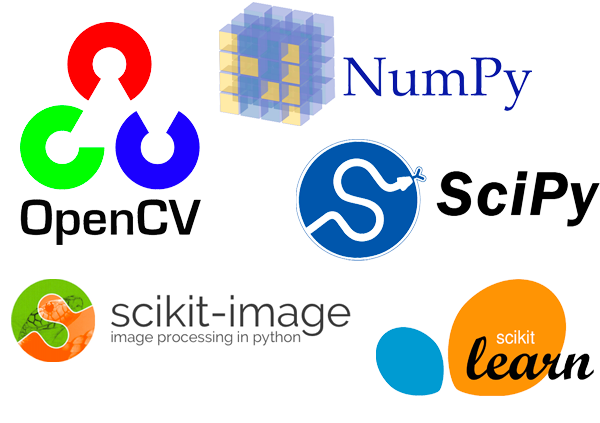
\includegraphics[width=0.3\textwidth]{python}
	\caption{Exemple de librairies Python.}
\end{figure}

\section{Les descripteurs d’image utilisés}
La première étape de création d'un système CBIR est le choix d'un descripteur pour indexer les images. \\
Pour la création de notre vecteur descripteur (signature), nous avons utilisé des caractéristiques de bas niveau comme déjà spécifier dans le chapitre 2. L'extraction se fait selon l'attribut visuel choisi: couleur, texture ou forme.
\subsection{Les descripteurs de couleur}
\textbf{Les modèles de couleur: }
Dans notre système, nous avons intégré l'espace RGB et l'espace TSV (HSV):\\

\begin{itemize}
	\item Le modèle TSV (Teinte Saturation Valeur) : est une représentation physique de la couleur, cet espace présente l’avantage de simuler le comportement visuel humain.
	
	\item Le modèle RVB (Rouge, Vert, Bleu) : est l’espace de couleur le plus utilisé pour la représentation de la couleur. L’avantage d’utiliser ce modèle est que cette représentation est extrêmement basique, puisqu’aucun traitement n’est nécessaire.\\
	
\end{itemize}

Notre système présente à l'utilisateur les descripteurs suivants :
\begin{itemize}
	\item L'histogramme (RGB et HSV),
	\item Les moments statistiques.
\end{itemize}

\subsubsection{Histogramme}
\paragraph{RVB (RGB):}
Dans la création de l’application, nous avons choisi d’utiliser les histogrammes par bloc dans l’espace RVB comme une technique de base comme spécifier dans l'article [Abed15].
On a choisi de diviser l'histogramme en 17 blocs pour chaque composante; Rouge, Verte et Bleu. Le vecteur de caractéristiques $ V_{histRGB} $ est généralement de taille 17x17x17 = 4913.
\begin{table}[H]
	\centering
	\caption{Exemple d'histogramme par blocs}
	\begin{tabular}{|c|c|c|c|c|c|}
		\hline
		\textbf{Block} & \textbf{Fréquence} & \textbf{Block} & \textbf{Fréquence} & \textbf{Block} & \textbf{Fréquence}\\
		\hline
		
		\makecell{0-15 } & \makecell{454 } & \makecell{16-30 } & \makecell{2324 }   & \makecell{31-45 } & \makecell{345 }   \\
		\hline
		
		\makecell{46-60 } & \makecell{903 } & \makecell{61-75 } & \makecell{133 }   & \makecell{76-90 } & \makecell{563 }   \\
		\hline
		
		\makecell{91-105 } & \makecell{123} & \makecell{106-120 } & \makecell{67 }   & \makecell{121-135 } & \makecell{124 }   \\
		\hline
		
		\makecell{136-150 } & \makecell{856} & \makecell{151-165 } & \makecell{45 }   & \makecell{166-180 } & \makecell{454 }   \\
		\hline
		
		\makecell{181-195 } & \makecell{355} & \makecell{196-210} & \makecell{31}   & \makecell{211-215 } & \makecell{4546 }   \\
		\hline
		
		\makecell{216-230 } & \makecell{456} & \makecell{231-255} & \makecell{3456}   & \makecell{  } & \makecell{  }   \\
		\hline
	\end{tabular}
	
	
\end{table}
\paragraph{TSV (HSV):}
Pour notre moteur de recherche d'images, nous utiliserons un histogramme couleur 3D dans l'espace couleur HSV avec 8 blocs pour le canal teinte, 12 blocs pour le canal saturation et 3 blocs pour le canal valeur en divisant l'image en 5 régions, ce qui donne un vecteur de caractéristiques $ V_{histHSV} $ est de  dimension 8 x 12 x 3 x 5 = 288 x 5 = 1440.
\begin{figure}[H]
	\centering
	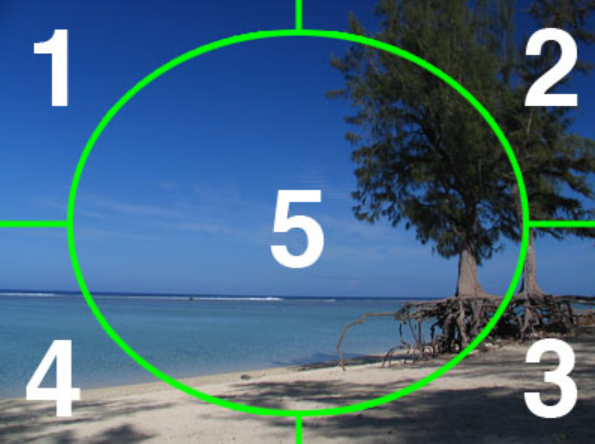
\includegraphics[width=0.3\textwidth]{5regions}
	\caption{Exemple de division d'une image en 5 régions différentes [Site01].}
\end{figure}
\subsubsection{Les moments de couleur}
Pour enrichir les index de la couleur, nous avons utilisé les moments de couleur au lieu de calculer la distribution complète comme pour les histogrammes. Dans cette étape, nous avons calculé les trois premiers moments de couleur (la moyenne, l’écart-type et le moment d'ordre 3) pour chaque canal (R,G,B) dans le but de garder seulement les neuf valeurs obtenues, ainsi le vecteur de caractéristiques $ V_{moments} $ est de tailles 9.

\subsection{Les descripteurs de texture}
Pour caractériser la texture, nous avons choisi l'un des descripteurs classiques à savoir les mesures de Haralick basé sur les matrices de co-occurrence. De plus, nous avons intégré les filtres de Gabor comme étant l'un des descripteurs fortement utilisés dans la littérature.
\subsubsection{Les mesures de Haralick}
Les mesures de Haralick sont calculées à partir de la matrice de co-occurrence de l'image. Haralick décrit 14 statistiques qui peuvent être calculées à partir de la matrice de co-occurrence dans le but de décrire la texture de l'image [Site02]. Nous adoptant l'implémentation de la librairie Mahotas [Site03] qui met en œuvre seulement les 13 premières mesures. La dernière (14ème) est normalement considérée comme instable. Alors, le vecteur de caractéristiques $ V_{Haralick} $ est de taille 13.

\subsubsection{Les filtres de Gabor}
Dans le but d'améliorer les performances lié à la recherche basé sur la texture, nous avons utilisé les filtres de Gabor vue leurs robustesse prouvé par de nombreuse travaux de recherche dans la littérature [ElHasnaoui17] et [ZZ18].\\

En traitement d'images, un filtre de Gabor, nommé d'après Dennis Gabor, est un filtre linéaire utilisé pour l'analyse de la texture:

\begin{equation}
g(x,y;\lambda,\theta,\psi,\sigma_x,\sigma_y) = \frac{1}{2\pi \sigma_x \sigma_y} \exp\left(\frac{-x'^2}{\sigma_x^2} + \frac{y'^2}{\sigma_y^2}\right)\exp\left(i\left(2\pi\frac{x'}{\lambda}+\psi\right)\right) 
\end{equation}
Où: $ x' = x \cos\theta + y \sin\theta\, $, $ y' = -x \sin\theta + y \cos\theta\, $, \\
$\psi$ : La phase, \\
$\theta$ : la direction, \\
et $ \lambda $: la fréquence.\\

Les filtres d'ondelettes de Gabor s'étendent sur 5 fréquences : 0.06, 0.09, 0.13, 0.18, 0.25 avec huit orientations $ \theta_0 = 0, \theta_n = \theta_{n-1} + \frac{\pi}{8} , n = 1,...,7$  et qui sont appliqués sur l'image. La moyenne et l'écart-type des coefficients d'ondelettes de Gabor des images résultante sont utilisés pour former un vecteur de caractéristiques $ V_{Gabor} $ de taille 5x8x2 = 240.

\subsection{Les descripteurs de forme}
Dans la partie basé sur la forme, nous avons intégré les moments de Hu comme descripteur classique et les moments de Zernike qui constitue une amélioration de performance comparant au moment de Hu.
\subsubsection{Moments de Hu}
Les moments de Hu sont basés sur les moments géométriques discutés dans le chapitre II section 2.2.3.\\
Si ƒ(x, y) est une image numérique, alors l'équation précédente devient:
\begin{equation}
\mu_{p,q} = \sum_{x=0}^{M-1}\sum_{y=0}^{N-1} (x- \bar{x})^p (y-\bar{y})^q f(x, y)
\end{equation}
D'où les moments géométriques (centraux):
\begin{figure}[H]
	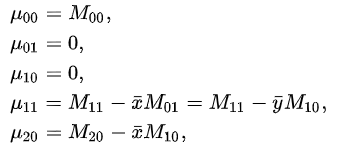
\includegraphics[width=0.5\textwidth]{momentCent} 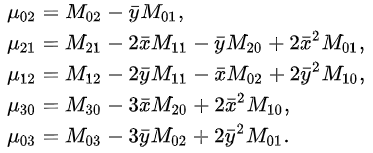
\includegraphics[width=0.5\textwidth]{momentCent1}
\end{figure}
Où:
\begin{equation}
\begin{tabular}{cc}
$\bar{x} = \frac{M_{1,0}}{M_{0,0}}$ & $\bar{y} = \frac{M_{0,1}}{M_{0,0}}$
\end{tabular}
\end{equation}
Les moments $ \mu_{p,q} $ invariants en ce qui concerne à la fois la translation et l'échelle peuvent être construits à partir des moments géométriques en divisant par un moment central zéro-ième correctement mis à l'échelle :
\begin{equation}
\eta _{{ij}}={\frac  {\mu _{{ij}}}{\mu _{{00}}^{{\left(1+{\frac  {i+j}{2}}\right)}}}}\,\!
\end{equation}
où $ i + j \ge 2 $.
Comme le montre le travail de Hu, [Hu62] les invariants en matière de translation, d'échelle et de rotation peuvent être construits :
\begin{figure}[H]
	\centering
	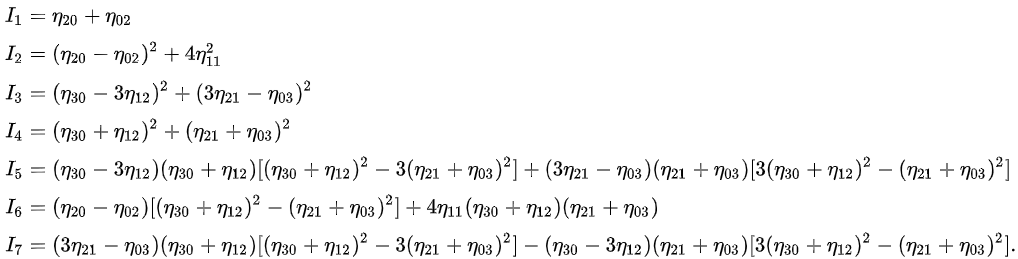
\includegraphics[width=1\textwidth]{huMom}
	\caption{Les moments de Hu.}
\end{figure}

Le vecteur de caractéristiques $ V_{Hu} $ est alors de taille 7.
\subsubsection{Moments de Zernike}
En 1934, Zernike [Site05] [MYB07] a proposé un ensemble de polynômes orthogonaux définis sur le cercle unité, à savoir les polynômes orthogonaux de Zernike, leur formule de définition est la suivante :
\begin{equation}
V_{mn}(x, y)~=~V_{mn}(r,\theta)~=~R_{mn}(r)\exp(jn\theta)
\end{equation}
où:
\begin{displaymath}
R_{mn}(r) = \sum_{s=0}^{\frac{m-\mid n \mid}{2}}(-1)^{s}~~F(m,n,s,r)
\end{displaymath}
\begin{displaymath}
F(m,n,s,r) = \frac{(m-s)!}{s!(\frac{m+\mid n \mid}{2}~-s)!~(\frac{m-\mid n \mid}{2}~-s)! }~r^{m-2s}
\end{displaymath}
$ R_{mn}(r) $  est le polynôme radial orthogonal, $ V_{mn}(x, y) $ est le polynôme orthogonal de Zernike, c'est un ensemble de fonctions orthogonales à valeurs complexes avec complétude définies sur le disque unité $x^{2} + y^{2} \leq ~1$ , n et m sont les ordres des polynômes orthogonaux de Zernike, où n est un entier positif ou zéro, m est un entier positif ou négatif, ils sont soumis aux conditions 
\begin{equation}
m- \mid n \mid ~=~pair~~,~~\mid n \mid~\leq~m
\end{equation}

\paragraph{Définition des Moments de Zernike:}
En 1980, sur la base des polynômes orthogonaux de Zernike, Teague [Teague80] a proposé pour la première fois la définition des moments de Zernike d'une fonction d'image f( x, y) en deux dimensions
\begin{equation}
Z_{mn} = \frac{m+1}{\pi} \int_{x} \int_{y} f(x,y)[V_{mn}(x,y)]^{*} ~dx~dy~~~~~\mbox{ avec $x^{2} + y^{2} \leq ~1$}
\end{equation}
où $m = 0,1,2,...,\infty$ et définit l'ordre, $f(x,y)$ est la fonction décrite et $*$ désigne le conjugué complexe. Alors que $n$ est un nombre entier (qui peut être positif ou négatif) décrivant la dépendance angulaire, ou rotation, sous conditions (4.4). Pour les images numériques, les intégrales sont remplacées par des sommations, alors les moments de Zernike sont réécrits comme :

\begin{equation}
Z_{mn} = \frac{m+1}{\pi} \sum_{x} \sum_{y} P_{xy}[V_{mn}(x,y)]^{*} ~~~~~\mbox{ avec $x^{2} + y^{2} \leq ~1$}
\end{equation}
Dans la littérature on trouve d'autres variants ou améliorations des moments de Zernike. Pour nous, on a adopter l'implémentation de la librairie Mahotas pour nous simplifier la vie. On générale, il faut fixer un rayon centré sur le centre de masse de l'image (le rayon du cercle enveloppant minimal de la forme).
Le vecteur de caractéristiques $ V_{Zernike} $ et de taille 25.

\subsection{Combinaison des descripteurs}
Les attributs: couleur, texture, forme décrivent les images par leur contenu visuel. La combinaison de ces attributs peut caractériser mieux le contenu. Il est donc intéressant de
combiner ces différents attributs pour une recherche plus efficace et plus discriminante. Les problèmes qui se posent lors de la combinaison de ces différents attributs pour la recherche et l’indexation sont au moins de trois ordres :

\begin{itemize}
	\item  \textbf{L'espace de description} : Le choix de l'espace de description consiste à rechercher les attributs visuels significatifs de la base de données d'images, l'ensemble de ces
	attributs étant représenté par un nuage de points dans un espace dimensionnel haut, alors les vecteurs contiennent plusieurs attributs, un problème qui se pose est celui de la dimension de l'espace de description. Ce problème est connu dans la communauté
	des bases de données par la malédiction de la dimension, lorsque le nombre de dimensions augmente, le volume de l'espace croît rapidement si bien que les données se retrouvent isolées et deviennent éparses.
	
	\item \textbf{ La mesure de la similarité} : Il s'agit d'une étape essentielle dans tout système de
	recherche. Dans le cas où les images sont décrites par différents attributs, une solution
	classique pour mesurer la similarité est de calculer séparément les mesures de
	similarité pour chaque attribut et de déduire ensuite une mesure composite de la
	similarité globale entre les images. Cela suppose évidemment que les différents
	attributs sont indexés séparément (avec des structures d'index séparées). Dans la base
	de données, il y a peu de méthodes qui utilisent plusieurs index pour structurer les
	données. Une autre difficulté liée à la similitude est de déterminer comment combiner
	plusieurs mesures souvent définies sur des domaines différents, avec des dynamiques
	différentes, des degrés d'importance différents, surtout pour l'utilisateur, mais aussi de
	natures différentes.
	
	\item \textbf{Structuration} : la phase de construction d'une structure d'index est une étape utile dans
	le cas où les données sont volumineuses et appartiennent à un grand espace de
	description. Il s'agit de structurer les nuages de points relatifs aux descripteurs des
	images et de les stocker efficacement dans une machine. Cette tâche de structuration
	peut s'avérer difficile dans le cas où les données à structurer sont de nature hétérogène.
	La difficulté réside dans le choix de la distance à utiliser pour structurer (mise en place
	d'un index) et dans la standardisation des différents types de données.
\end{itemize}
\subsubsection{La couleur et la texture}
Pour diminuer la taille du vecteur descripteur (signature) autant que possible nous avons choisi d'utiliser les moments de couleur, qui produit une signature de taille 9, pour caractériser la couleur. En ce qui concerne la caractérisation de la texture on travaille avec les filtres de Gabor.
\begin{figure}[H]
	\centering
	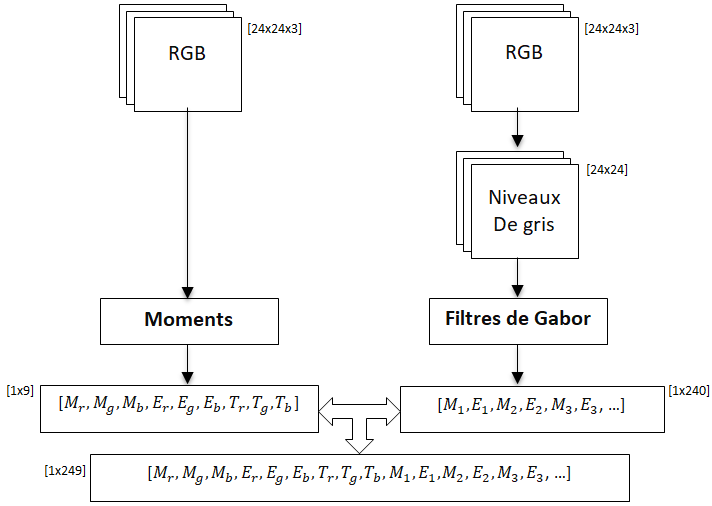
\includegraphics[width=0.6\textwidth]{clrtxtr}
	\caption{Dérivation de signature couleur et texture.}
\end{figure}
Où: 
M: Moyenne, E: Ecart-type, T: moment d'ordre trois.
\begin{equation}
V_{final} = V_{moments} \bigcup V_{Gabor}
\end{equation}
\subsubsection{La couleur et la forme}
Nous utilisons les moments de couleur pour les mêmes raisons pour caractériser la couleur. En ce qui concerne la caractérisation de la forme on travaille avec les moments de Zernike car l'expérience preuve qu'il sont plus performant que les moments de Hu.
\begin{figure}[H]
	\centering
	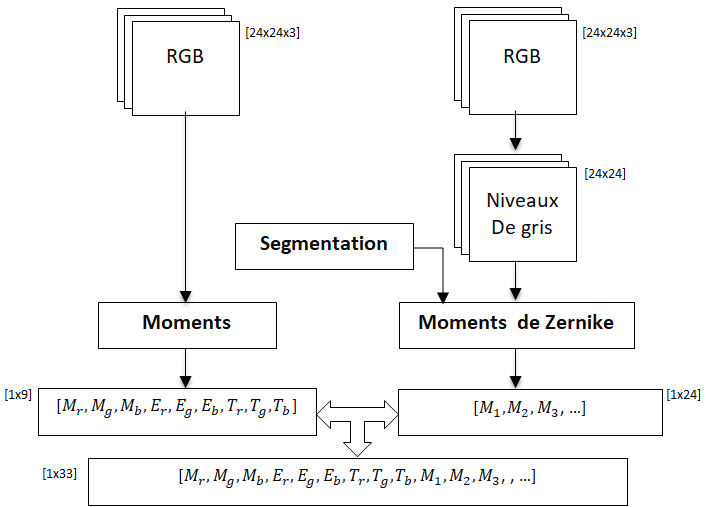
\includegraphics[width=0.6\textwidth]{clrshp}
	\caption{Dérivation de signature couleur et texture.}
\end{figure}
Où: 
$ M_i $: Moment i.
\begin{equation}
V_{final} = V_{moments} \bigcup V_{Zernike}
\end{equation}

Pour fusionner les différents descripteurs, une méthode utilisée dans différents travaux [ElAsnaoui17] consiste à pondérer les distances de similarité. Ainsi les descripteurs pertinents pour la recherche se verront attribuer des poids les plus importants, et auront donc plus d’influence dans le résultat final. La combinaison des distances est donnée par la relation suivante :
\begin{equation}
	D_{global}(Q, I) = w_1 \times 	D_{1}(Q, I) + w_2 \times 	D_{2}(Q, I)
\end{equation}
où $ w_i $ est un poids qui prend une valeur entre 0 et 1 avec $ w_1+w_2= 1 $.
\section{Mesures de similarité}
La deuxième étape dans les systèmes de recherche d'image par le contenu est le choix d'une mesure de similarité pour effectuer la recherche.\\

Pour rechercher les images les plus similaires à une image requête, il faut pouvoir mesurer la similarité entre les images. Lorsqu’un utilisateur lance une recherche, le système effectue une mesure entre le signature de la requête et les signatures des images de la base dans l’espace des attributs (signatures).\\

D'une façon générale, nous avons choisi d’utiliser les distances dérivées de la famille de distances de Minkowski; la distance de Manhatan et la distance Euclidienne.\\

Pour les distributions statistiques à savoir les histogrammes, nous avons ajouter les distances:  $\chi^2$ (CHI-square) et Bhattacharyya  .

\begin{table}[H]
	\centering
	\caption{Les distances de Minkowski}
	\begin{tabular}{|c|c|c|}
		\hline
		\textbf{Distance} & \textbf{Formule}\\
		\hline
		\makecell{Manhatttan } & \makecell{\\
			$  d_1(I_1, I_2) = \sum_{i=1}^{N} \left|{I}_{1}(i)-{I}_{2}(i)\right|  $ }   \\
		\hline
		
		\makecell{Euclidienne} & \makecell{\\ $ d_2(I_1, I_2) =  \sqrt{\sum_{i=1}^{N} \left|{I}_{1}(i)-{I}_{2}(i)\right|^2} $}   \\
		\hline
		
		\makecell{$\chi^2$ (CHI-square)  } & 
			\makecell{\\
				$d(I_1, I_2)=\sum_{i=1}^{N} \frac{(I_1(i)-I_2(i))^2}{I_1(i)}$
			} \\   
		\hline
		
		\makecell{Bhattacharyya } & 
		\makecell{\\
			$d(I_1, I_2) ~=~ \sqrt{ 1 - \frac{1}{ \sqrt{\bar{I_1}\bar{I_2} N^2} }  \sum_{i=1}^{N} \sqrt{I_1(i)\times I_2(i)}}$
		} \\   
		\hline
		
		
	\end{tabular}
	
\end{table}
Ou :\\
$ I_1, I_2 $ sont les deux vecteurs de caractéristiques.\\
$ N $ est la dimension de vecteur.\\
$ i $ indice.
$ bar{I_i} $ la moyenne.

\section{Les bases d’mages utilisées }
\textbf{Corel-1000 - Wang:}
Cette base d’images contient 1000 images en couleurs. Ces images ont
été divisées en 10 classes de 100 images. Les thèmes représentés par les 10 classes sont : monuments, plage, autobus, dinosaures, aliments, éléphants, fleurs, chevaux, montagnes et l’Afrique.

\begin{figure}[H]
	\centering
	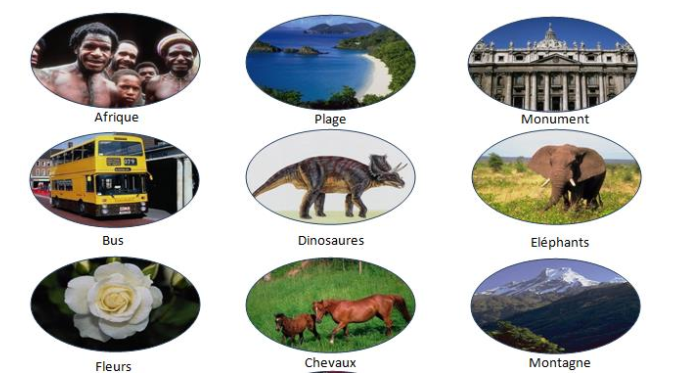
\includegraphics[width=0.6\textwidth]{wang} 
	\caption{Quelques images de la base d’image WANG.}
\end{figure}

\textbf{Columbia Object Image Library (COIL-100):}
Cette base d’images est très connue pour la reconnaissance des objets. Il y a deux bases d’images COIL : COIL-20 qui contient des images en niveaux de gris prises à partir de 20 objets différents et COIL-100 qui contient des images en couleurs prises à partir de 100 objets différents. Les deux bases d’images consistent en des images prises à partir des objets 3D avec des positions différentes. La base COIL-100 a 7200 images en couleurs (100 objets x72 images/objet). Chaque image a une taille de 128x128 pixels.

\begin{figure}[H]
	\centering
	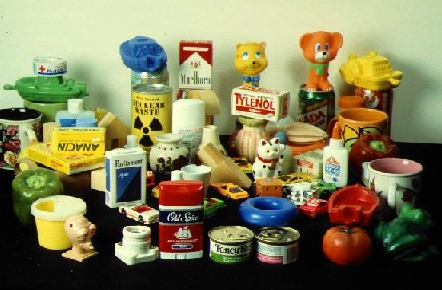
\includegraphics[width=0.6\textwidth]{coil} 
	\caption{Objets utilisés dans COIL-100.}
\end{figure}

\textbf{Columbia-Utrecht Reflectance and Texture Database (CuRRET):}
Des chercheurs des universités de Columbia et d'Utrecht ont collaboré dans une étude approfondie de l'aspect visuel des surfaces du monde réel. Cet effort conjoint, parrainé en partie par REALISE de la Commission européenne, la National Science Foundation et par le DARPA/ONR dans le cadre de la subvention MURI n° N00014-95-1-0601, a donné lieu à 3 bases de données [Site04]. Nous avons choisi 33 échantillons parmi 61 échantillons avec 50 images par échantillon.
\begin{figure}[H]
	\centering
	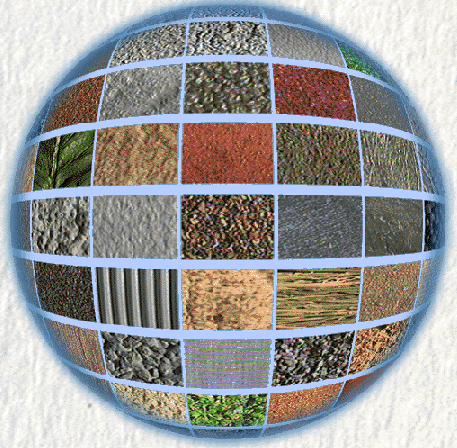
\includegraphics[width=0.5\textwidth]{curet} 
	\caption{Quelques images de la base d’image CuRRET.}
\end{figure}

%\textbf{MIT1995 - VisTex:}
%La base de données VisTex est une collection d'images de texture. La base de données a été créée dans le but de fournir un large ensemble de textures de haute qualité pour les applications de vision par ordinateur. En particulier, l'ensemble a été conçu comme une alternative à la bibliothèque de textures Brodatz, qui n'est pas disponible gratuitement pour la recherche [Site01]. L'objectif de VisTex est de fournir des images de texture qui sont représentatives des conditions du monde réel. Si VisTex peut remplacer les collections de textures traditionnelles, il comprend des exemples de nombreuses textures non traditionnelles. La base de données comporte plus de 100 images.
%
%\begin{figure}[h]
%	\centering
%	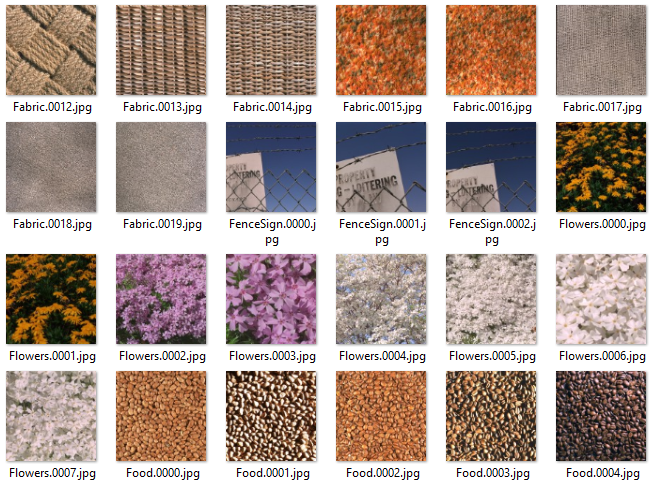
\includegraphics[width=0.6\textwidth]{VisTex} 
%	\caption{Quelques images de la base d’image VisTex.}
%\end{figure}
%
%\textbf{MIT1995 - TRUNK12:}
%Comme il n'existe pas d'ensemble de données d'images d'écorces d'arbres connu et accessible au public, un nouvel ensemble de données accessible au public a été créé dans le cadre de la thèse de Bsc [Site02]. Il contient environ 360 images d'écorces de 12 arbres différents qui se trouvent en Slovénie. Chaque classe d'arbres comprend environ 30 images au format JPEG, avec une résolution de 3000 x 4000 pixels. Toutes les images ont été prises avec l'appareil photo Nikon COOLPIX S3000 dans les mêmes conditions (distance de 20 cm, plusieurs arbres par classe, en évitant le bruit comme la mousse, mêmes conditions de lumière, prises en position verticale).
%
%\begin{figure}[H]
%	\centering
%	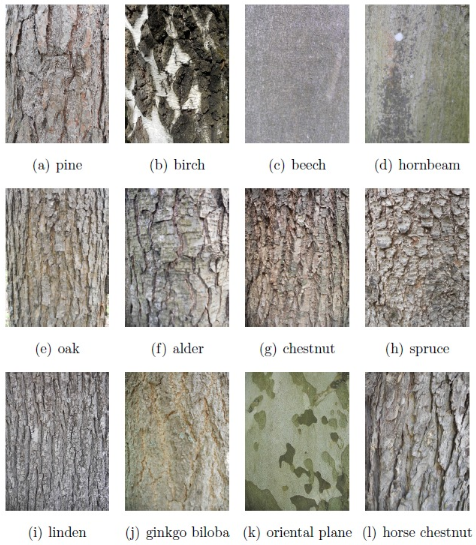
\includegraphics[width=0.6\textwidth]{trunk} 
%	\caption{Quelques images de la base d’image TRUNK12.}
%\end{figure}

\section{Mesure de la qualité des réponses}
Dans les systèmes de recherche d’images, une image est pertinente pour
une requête si les deux images sont dans la même classe.
La précision (ou valeur prédictive positive) est la proportion des items pertinents parmi l'ensemble des items proposés; le rappel (ou sensibilité) est la proportion des items pertinents proposés parmi l'ensemble des items pertinents. Ces deux notions correspondent ainsi à une conception et à une mesure de la pertinence.\\

Lorsqu'un moteur de recherche, par exemple, retourne 30 pages web dont seulement 20 sont pertinentes (les vrais positifs) et 10 ne le sont pas (les faux positifs), mais qu'il omet 40 autres pages pertinentes (les faux négatifs), sa précision est de 20/30 = 2/3 et son rappel vaut 20/(20+40) = 1/3.\\

La précision peut ainsi être comprise comme une mesure de l'exactitude ou de la qualité, tandis que le rappel est une mesure de l'exhaustivité ou de la quantité.\\


\begin{figure}[H]
	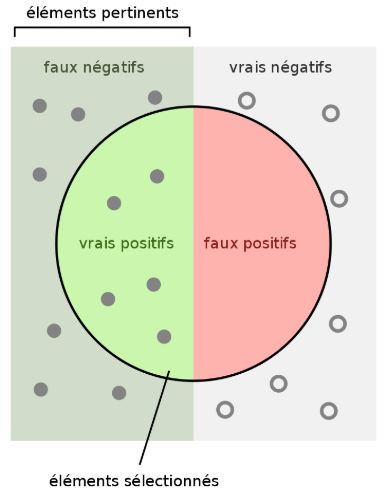
\includegraphics[width=0.5\textwidth]{recpre} 
	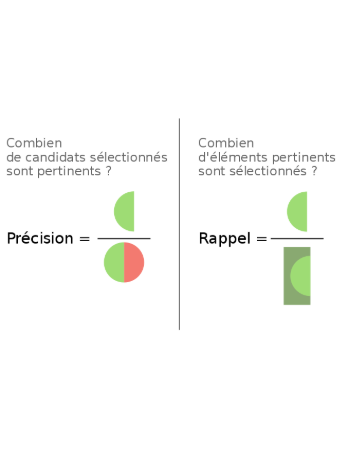
\includegraphics[width=0.5\textwidth]{recallprecision} 
	\caption{Rappel et précision comme illustré par Wikipédia.}
\end{figure}
Le rappel et la précision sont deux mesures très utilisées pour l’évaluation des performances d’un système CBIR. 

\begin{equation}
R = \frac{\text{VP}}{\text{FN et VP}} = \frac{\text{Nombre d'images pértinentes retrouvées} }{\text{Nombre total d'images pértinentes}}
\end{equation}
\begin{equation}
P = \frac{\text{VP}}{\text{VP et FP}} = \frac{\text{Nombre d'images pértinentes retrouvées}}{\text{Nombre total d'images retrouvées}}
\end{equation}
Où: \\
VP: Vrais Positifs\\
VN: Vrais Négatifs\\
FP: Faux Positifs\\
FN: Faux Négatifs.
 
En statistique, la précision est appelée valeur prédictive positive et  le rappel est appelé sensibilité.\\

D'après ses deux mesures on peut déduire un troisième qu'on appelle F-mesure ou F-score. Une mesure qui combine la précision et le rappel est leur moyenne harmonique:
\begin{equation}
F = \frac{2\times R\times P}{R + P} 
\end{equation}
La F-mesure correspond à un compromis de la précision et du rappel donnant la performance du système.\\

Il faut noter que nous avons ajouter la possibilité d'afficher la matrice de confusion: une matrice qui mesure la qualité d'un système de classification. Chaque ligne correspond à une classe réelle, chaque colonne correspond à une classe estimée. 
\begin{figure}[H]
	\centering
	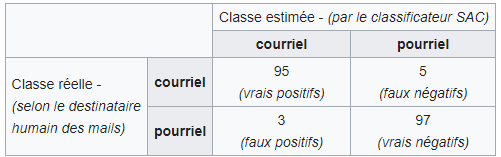
\includegraphics[width=0.7\textwidth]{Figures/cm.png} 
	\caption{Exemple d'une matrice de confusion (source: Wikipédia).}
\end{figure}
Le système contient une fenètre pour calculer la pértinance de chaque requête:
\begin{figure}[H]
	\centering
	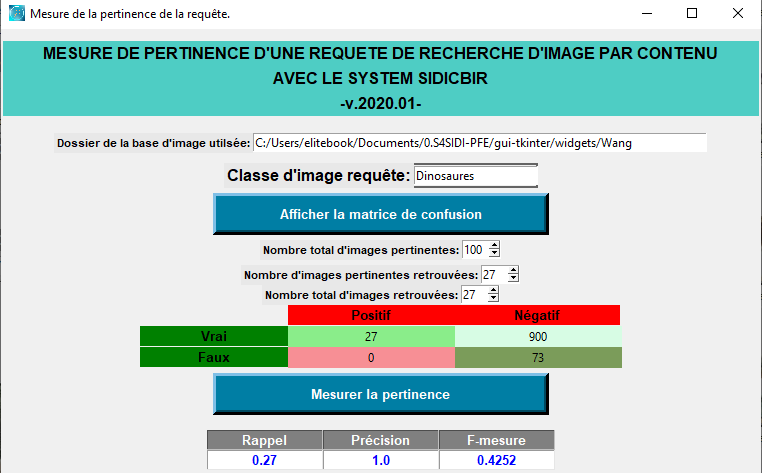
\includegraphics[width=0.6\textwidth]{mesures} 
	\caption{Exemple d'une matrice de confusion calculé par le système.}
\end{figure}
\section{Architecture de l’application}
Dans un système d’extraction d’images par le contenu il existe deux types de traitements :
\begin{itemize}
	\item \textbf{Traitement offline :}
	Ce type de traitement représente la phase de la construction de la base des signatures (d’attributs/vecteurs descripteurs).
	Cette opération est réalisée durant la construction du système.
	\item \textbf{Traitement online :}
	Ce type de traitement est effectué lors de l’introduction de la requête de l’utilisateur.
	Les signatures sont extraits de l’image requête puis comparés à ceux de la base de signatures qui a été déjà construite au préalable.
\end{itemize}
\begin{figure}[H]
	\centering
	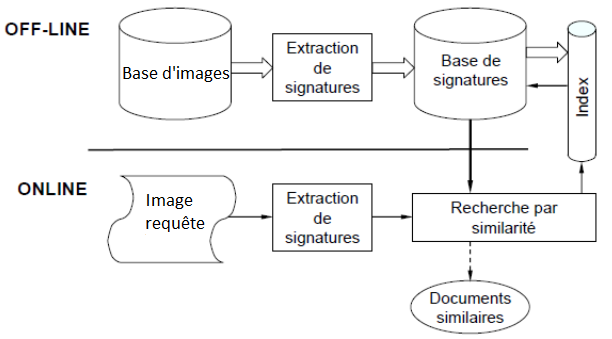
\includegraphics[width=0.9\textwidth]{architectureBDMM} 
	\caption{Architecture de l’application.}
\end{figure}

\begin{figure}[H]
	\centering
	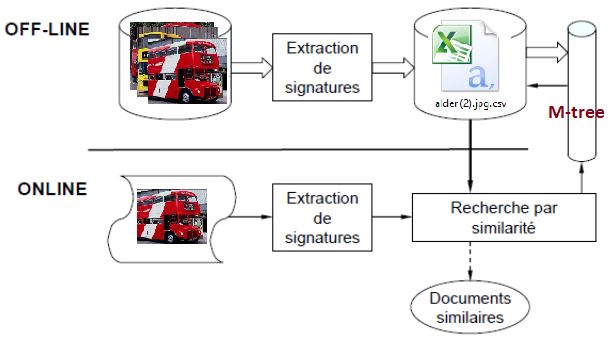
\includegraphics[width=0.9\textwidth]{architecture} 
	\caption{Architecture de l’application avec utiles utilisés.}
\end{figure}
\paragraph{La base de signatures:}
La base d’attributs ou signatures est constituée d’un ensemble de fichiers CSV (un fichier par image). Chaque fichier est constituée de $ n+1 $ champs :
\begin{itemize}
	\item 1 champ pour le chemin absolu de l'image (oid pour M-Tree),
	\item n champs de vecteurs descripteurs calculer par le descripteur.
\end{itemize}
\section{L’interface utilisateur }
Généralement, l'interface utilisateur de notre système permet à l'utilisateur des tâches comme:
 \begin{itemize}
 	\item Rechercher des images similaires à l'image requête (en ligne),
 	\item Indexer une bases d'images (hors ligne),
 	\item Calculer la qualité de chaque réponse ou requête,
 \end{itemize}

L'interface principale permet à l’utilisateur (Figure 4.8): 
\begin{itemize}
	\item d'indexer une bases d'images (phase hors ligne) ou una bases de signatures,
	\item d’introduire son image requête,
	\item de choisir le descripteur à utiliser avec le type d'images en cas d'indexation d'une base d'images,
	\item de choisir la mesure de similarité à utiliser,
	\item de rechercher des images similaires à l'image requête (en ligne),
	\item de visualiser les images indexer pour en sélectionner la requête,
	\item de calculer la qualité de chaque réponse ou requête,
	\item de consulte la fenêtre aide pour savoir comment utiliser le système...etc.
\end{itemize}

\begin{figure}[H]
	\centering
	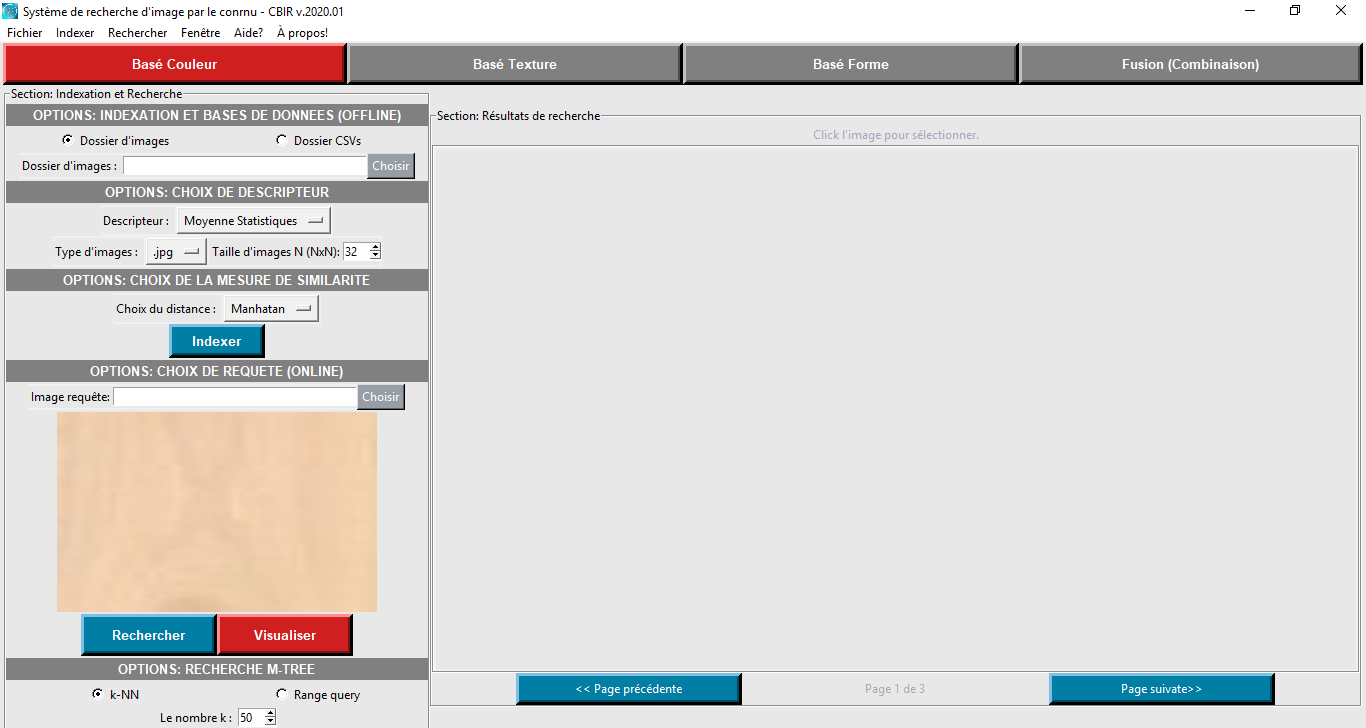
\includegraphics[width=0.9\textwidth]{gui} 
	\caption{L'interface d’utilisateur.}
\end{figure}

La section des options de l'indexation et la recherche change selon les attributs visuels choisis.

\begin{figure}[H]
	\centering
	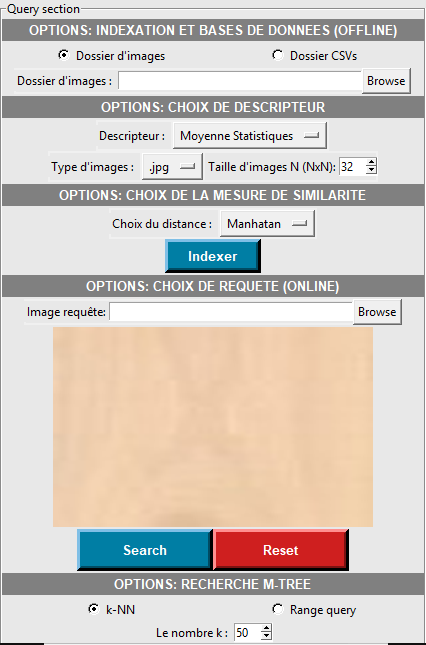
\includegraphics[width=0.35\textwidth]{baseC} \space
	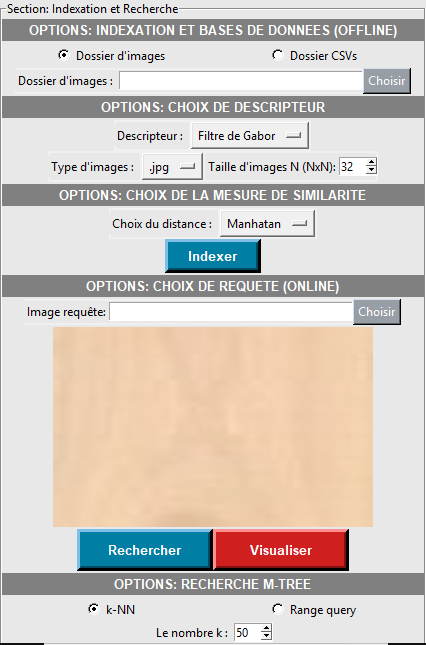
\includegraphics[width=0.35\textwidth]{baseT} 
	\caption{L'interface d’utilisateur, section requête: \\
	Gauche: basé couler, Droite: Basé texture.}
\end{figure}
\begin{figure}[H]
	\centering
	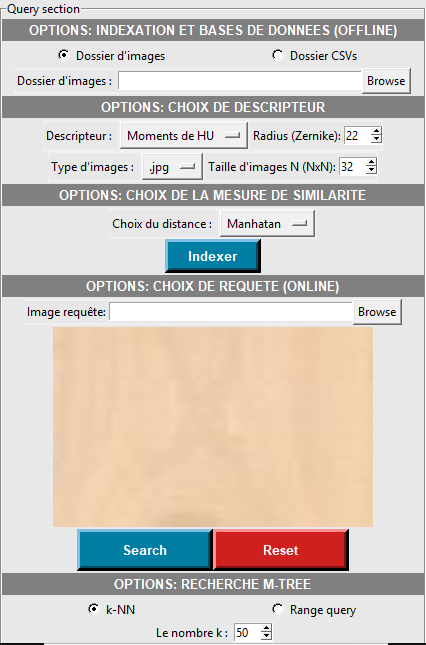
\includegraphics[width=0.35\textwidth]{baseF} \space
	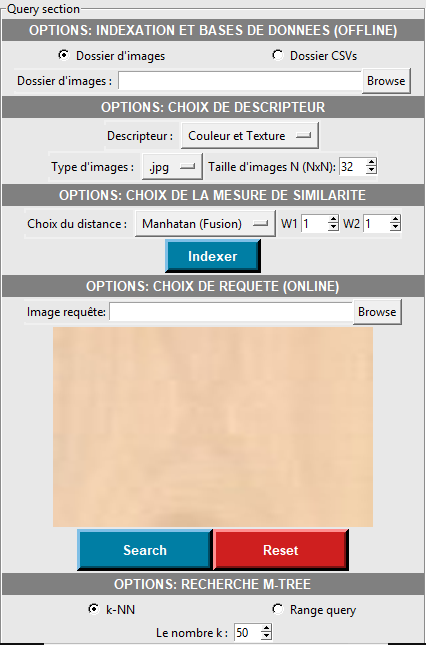
\includegraphics[width=0.35\textwidth]{baseCTS} 
	\caption{L'interface d’utilisateur, section requête: \\
		Gauche: basé forme, Droite: Basé fusion}
\end{figure}


Après avoir choisi la base à indexer et les autres paramètres relatives à l'étapes d'indexations (descripteur, type d'images et mesure de similarité) l’utilisateur indexe cette base en appuyant sur la bouton 'Indexer'. Ainsi, l'indexation commence. \\

\begin{figure}[H]
	\centering
	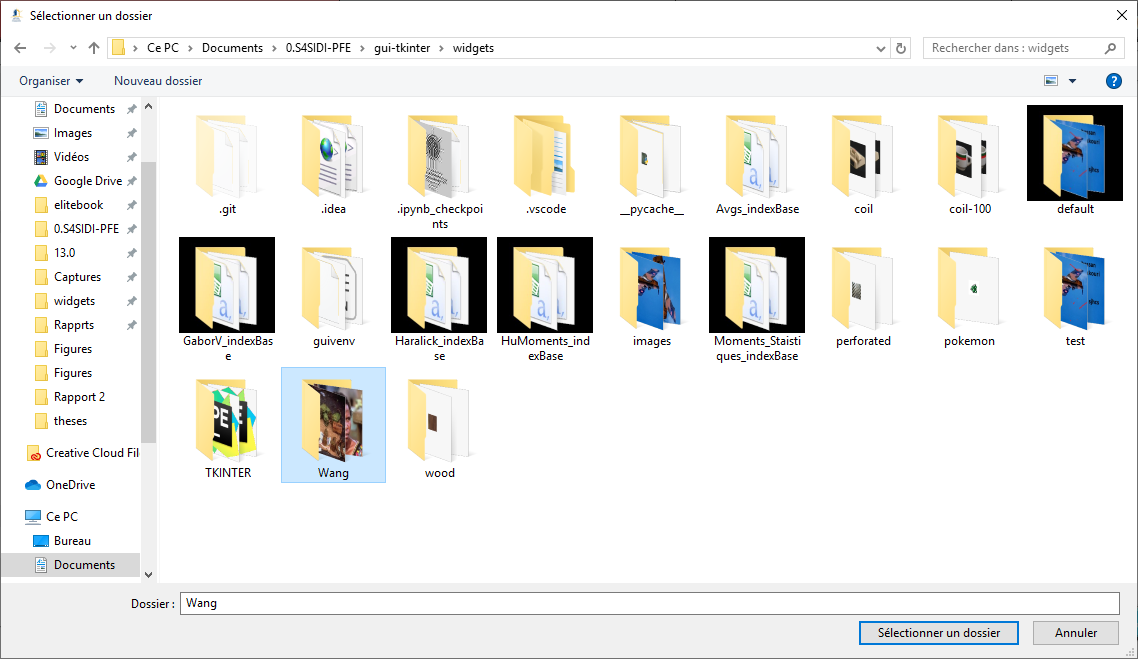
\includegraphics[width=0.7\textwidth]{browse folder} 
	\caption{Choix d'une base à indexer.}
\end{figure}

Une fois l'indexation est faite, l’utilisateur peut lancer une recherche après avoir choisi l'mage requête en appuyant sur la bouton 'Rechercher'. Pendant cette étape la signature de l’image est calculé pour l'utiliser dans l'un des requêtes de rechrche de la structure d'indexation M-Tree (Requête intervalle ou k-NN).\\

\begin{figure}[H]
	\centering
	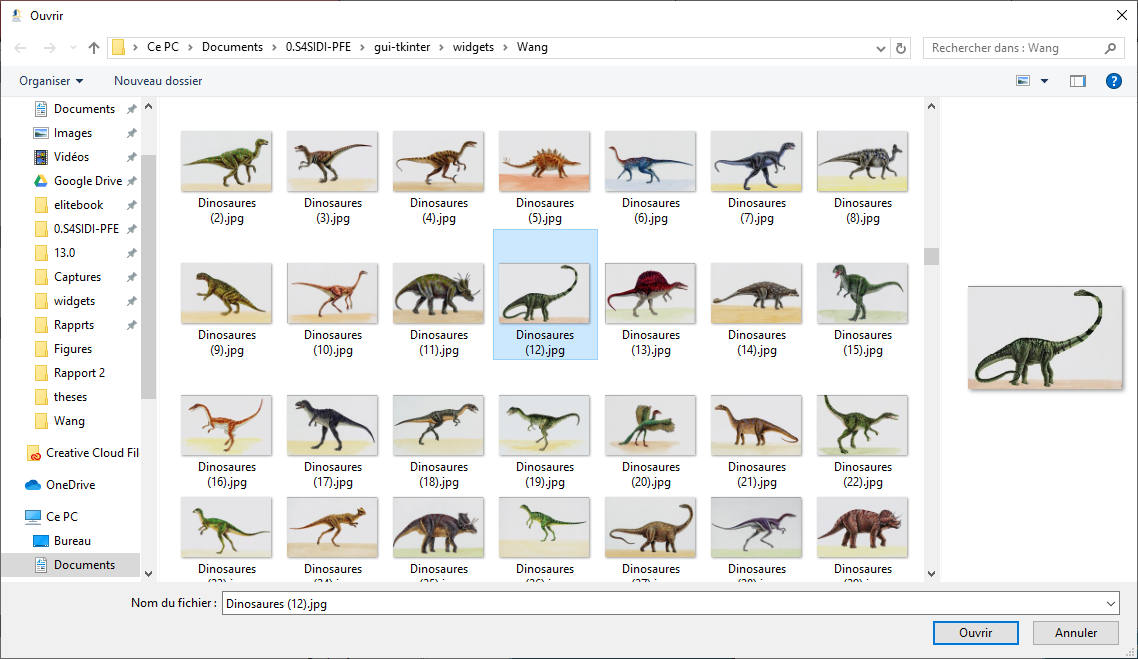
\includegraphics[width=0.7\textwidth]{browse query} 
	\caption{Choix de l'mage requête.}
\end{figure}
Résultas:
\begin{figure}[H]
	\centering
	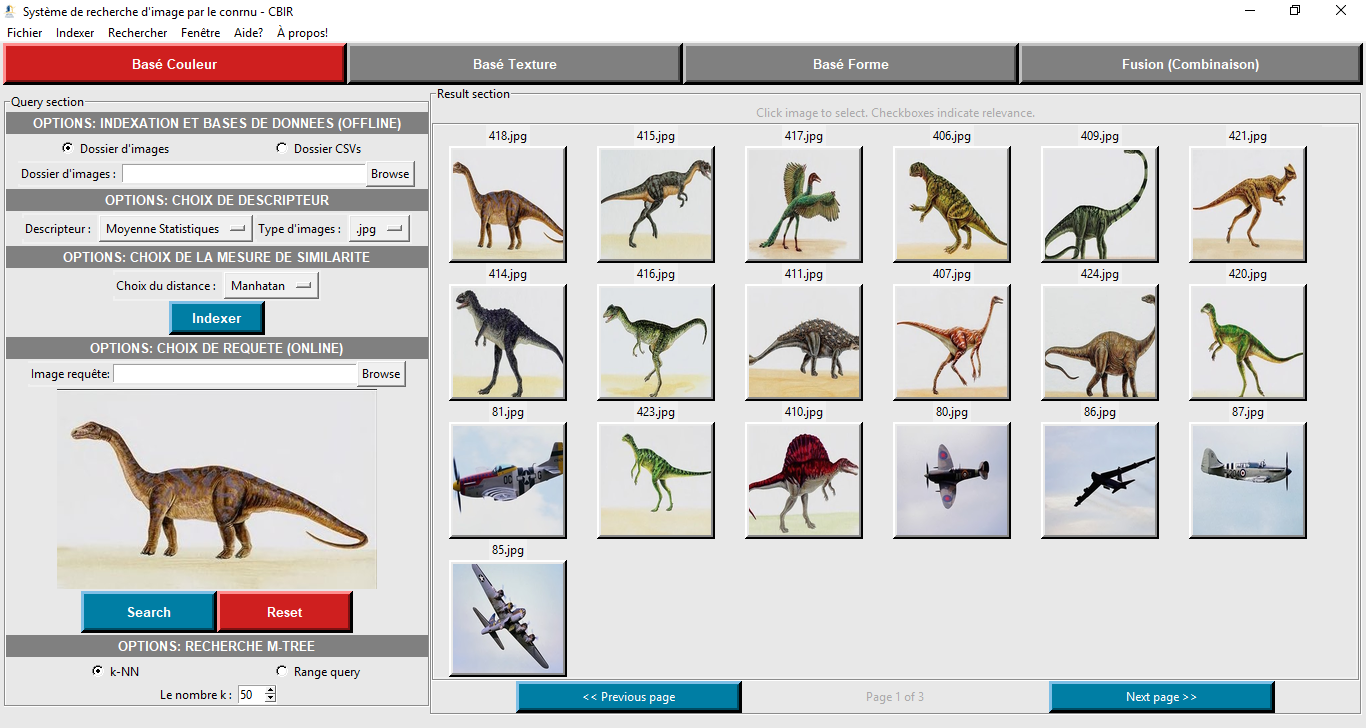
\includegraphics[width=0.7\textwidth]{query result} 
	\caption{Résultats de la recherche.}
\end{figure}

Le système affiche une liste d'images ordonnées par le degré de similarité.

Pour mesurer la qualité de la réponse on va vers le menu \textbf{fenêtre->mesures}:
\begin{figure}[H]
	\centering
	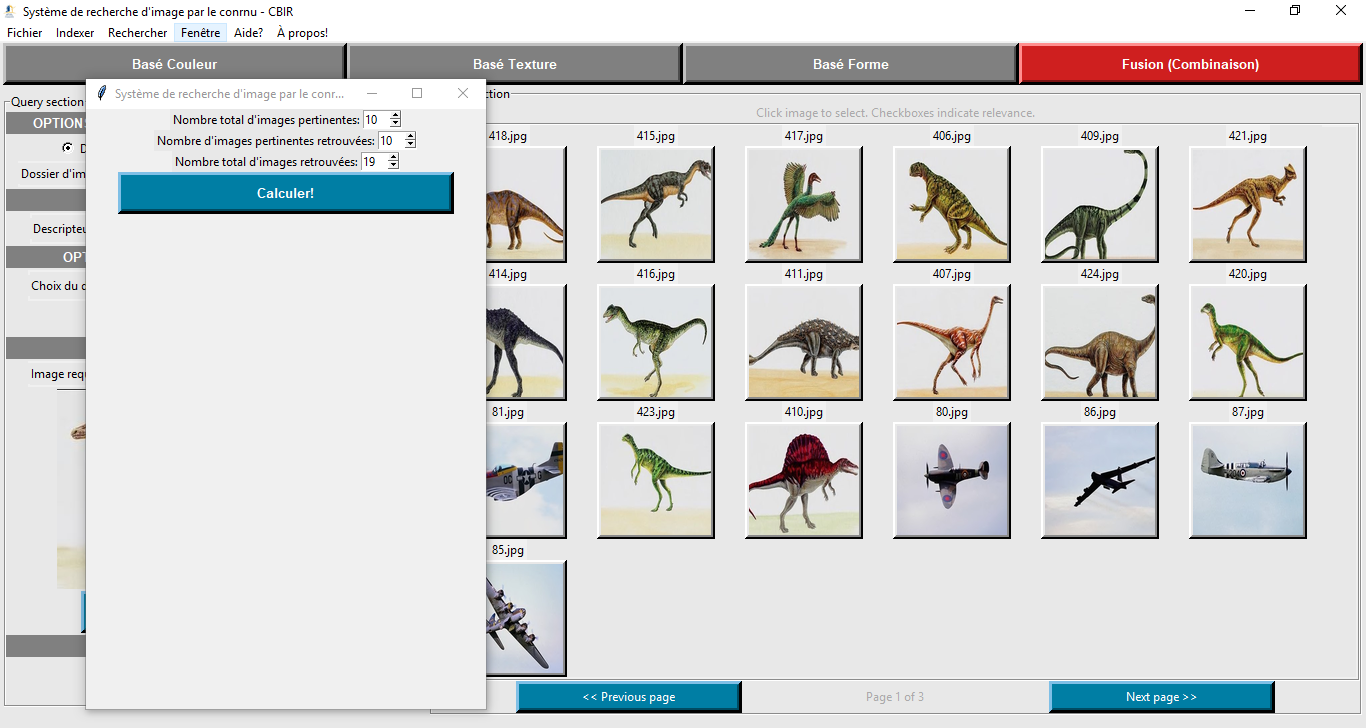
\includegraphics[width=0.7\textwidth]{mesuresQu} 
	\caption{La fenêtre des mesures de la pertinence.}
\end{figure}
On calcule:
\begin{figure}[H]
	\centering
	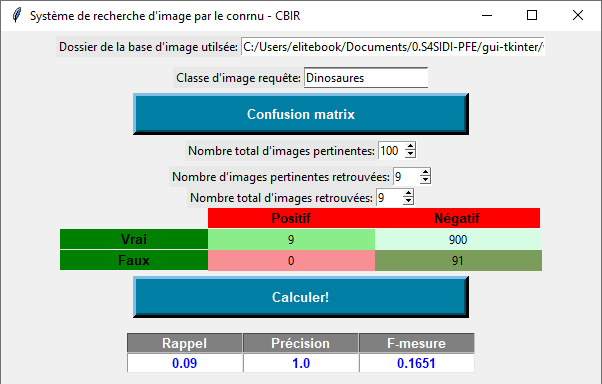
\includegraphics[width=0.7\textwidth]{QUresult} 
	\caption{Résultatsdes mesures de la pertinence.}
\end{figure}

\section{Évaluation de système}
Nous avons testé la performance de chaque descripteurs utilisé et dans cette section nous présenterons les différents résultats.

\paragraph{Processus suivi:}
Dans cette partie nous avons évalué l’application avec le calcule du rappel, la précision et F-mesure pour chaque image requête. Le principe de fonctionnement est simple; les images requêtes sont sélectionnées de manière aléatoires (sans répétition de la même image requête) et on calcul les mesures de pertinence. 
\subsection{Descripteurs de la couleur}
Pour cette section, nous avons effectué un ensemble de tests sur 50 images requêtes (5 images pour chaque classe) de la base Wang. Les mesures de chaque classe sont calculées par la moyenne de ses images. Puis à la phase finale, on peut déduire la précision globale de système qui représente la moyenne de toutes les classes. On travailler avec les mêmes requêtes pour les deux descripteurs.

\begin{figure}[H]
	\centering
	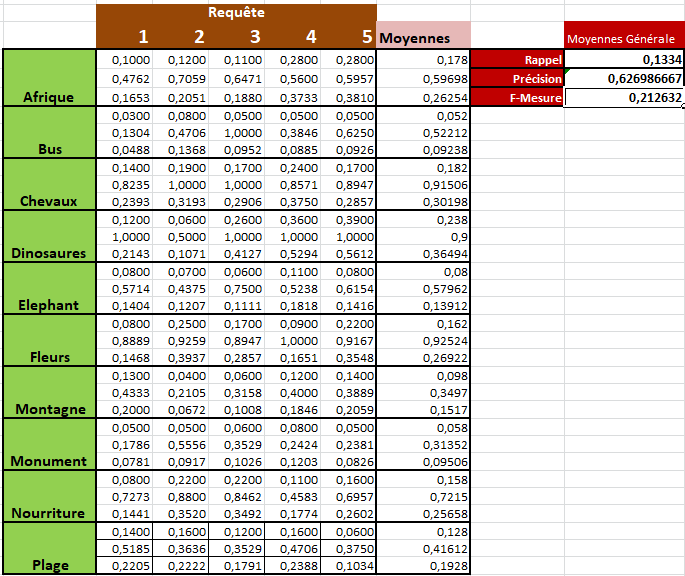
\includegraphics[width=.7\textwidth]{MomentsColPert} 
	\caption{Pertinence des moments de couleur.}
\end{figure}

\begin{figure}[H]
	\centering
	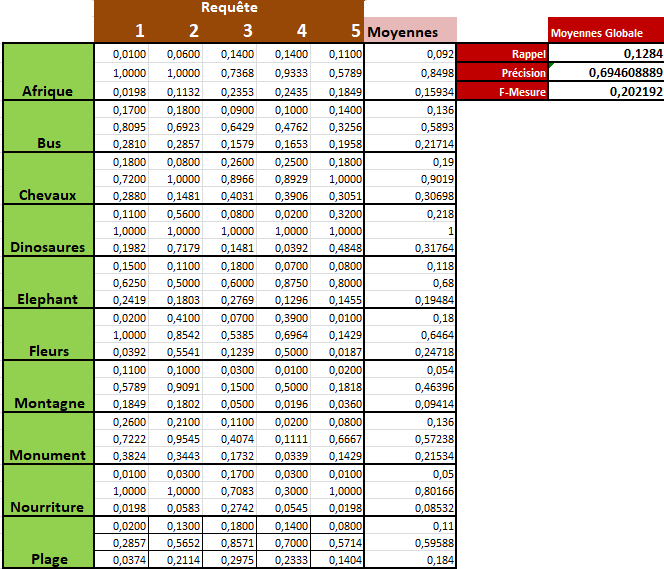
\includegraphics[width=.7\textwidth]{histRGBPert} 
	\caption{Pertinence de l'histogramme RGB.}
\end{figure}
On remarque, d'après les deux figures 4.22 et 4.23, que les résultats sont proches avec les deux descripteurs sauf que l'histogramme présente presque 0,70 en précision contre 0,63 pour les moments de couleur.
\subsection{Descripteurs de la texture}
Pour cette section, nous avons effectué un ensemble de tests sur 25 images requêtes de la base CuRRET avec la distance de Manhatan. On travaille avec les mêmes requêtes pour les deux descripteurs. 
On fixe les options comme suite:
\begin{figure}[H]
	\centering
	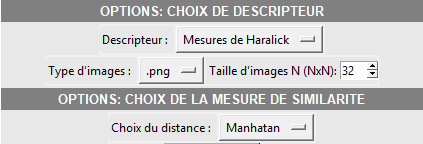
\includegraphics[width=.45\textwidth]{Haralick options} \space
	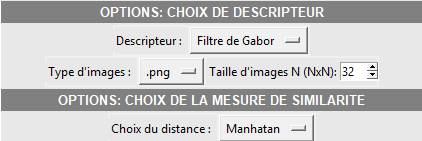
\includegraphics[width=.45\textwidth]{GaborOptions} 
	\caption{Options: des mesures de Haralick (Gauche),  des filtres de Gabor (Droite).}
\end{figure}
On obtient:
\begin{figure}[H]
	\centering
	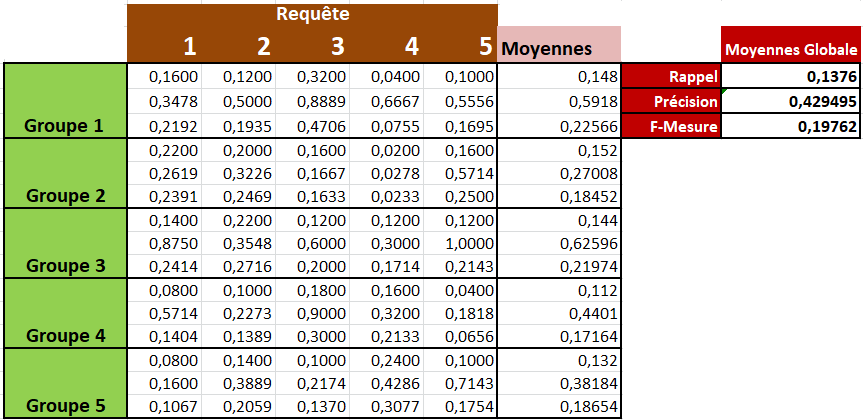
\includegraphics[width=.7\textwidth]{HaralickPert} 
	\caption{Pertinence des mesures de Haralick.}
\end{figure}



\begin{figure}[H]
	\centering
	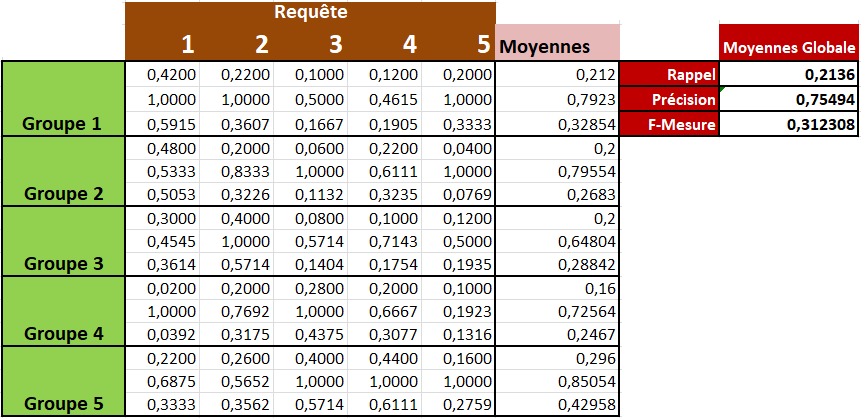
\includegraphics[width=.7\textwidth]{GaborPert} 
	\caption{Pertinence des filtres de Gabor.}
\end{figure}
Comme les résultats le montre, les filtres de Gabor présente des réponse de bonne qualité comparant aux mesures de Haralick (Comme le montre les figure 4.25 et 4.26, 75\% en précision pour Gabor contre 43\% pour Haralick). 
\subsection{Descripteurs de la forme}
Pour évaluer les descripteurs de la forme, nous avons effectué un ensemble de testes sur 25 images requêtes de la base COIL-100 avec la distance de Manhatan. On a travaillé avec les mêmes requêtes pour les deux descripteurs. Généralement, on effectue une segmentation des images avant d'extraire les informations.\\

On fixe les options comme suite:
\begin{figure}[H]
	\centering
	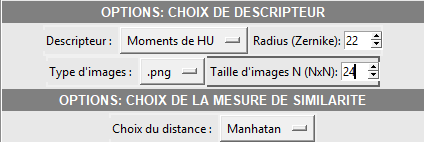
\includegraphics[width=.45\textwidth]{HuOptions} \space
	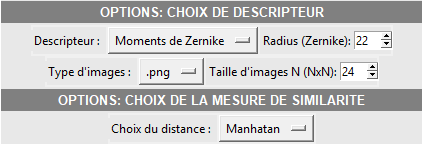
\includegraphics[width=.45\textwidth]{ZernikeOptions} 
	\caption{Options: des moments de Hu (Gauche), des moments de Zernike (Droite).}
\end{figure}
On obtient:
\begin{figure}[H]
	\centering
	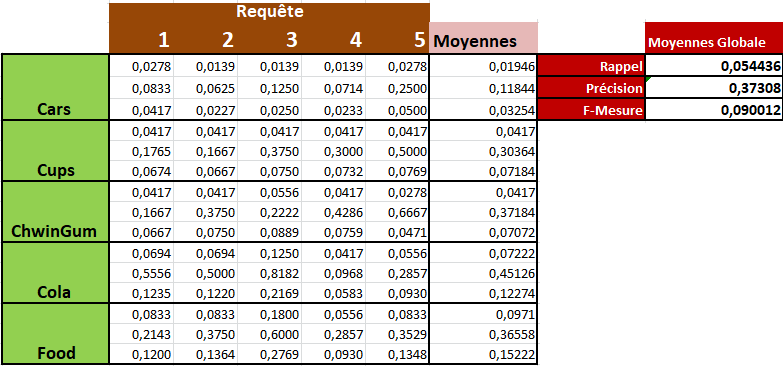
\includegraphics[width=.7\textwidth]{HuPert} 
	\caption{Pertinence des moments de Hu.}
\end{figure}

\begin{figure}[H]
	\centering
	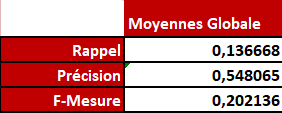
\includegraphics[width=.7\textwidth]{ZernikePert} 
	\caption{Pertinence des moments de Zernike.}
\end{figure}
On remarque que les moments de Zernike sont plus performant que les moments de Hu. Comme le montre les figures 4.28 et 4.29, les moments de Zernike donnent une précision de 55\% alors que ceux de Hu donnent seulement 37\%.
\subsection{Descripteurs combinés}
Dans cette partie nous travaillons avec les mêmes bases de données et mêmes images requêtes utilisés dans les deux parties précédentes; CuRRET pour la texture et COIL-100 pour la forme. Nous avons fixer $  0,5 $ pour les deux poids dans un premier temps.
\begin{figure}[H]
	\centering
	\includegraphics[width=.45\textwidth]{ColTxtrOptions2} \space
	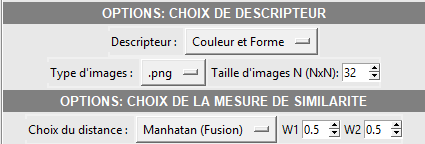
\includegraphics[width=.45\textwidth]{ColShpOptions} 
	\caption{Options des moments de couleur combiné avec les filtres de Gabor (Gauche), et des moments de couleur combiné avec les moments de Zernike (Droite).}
\end{figure}
On obtient:
\begin{figure}[H]
	\centering
	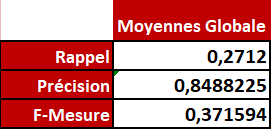
\includegraphics[width=.7\textwidth]{colTxtrPert} 
	\caption{Pertinence des moments de couleur combiné avec les filtres de Gabor.}
\end{figure}

\begin{figure}[H]
	\centering
	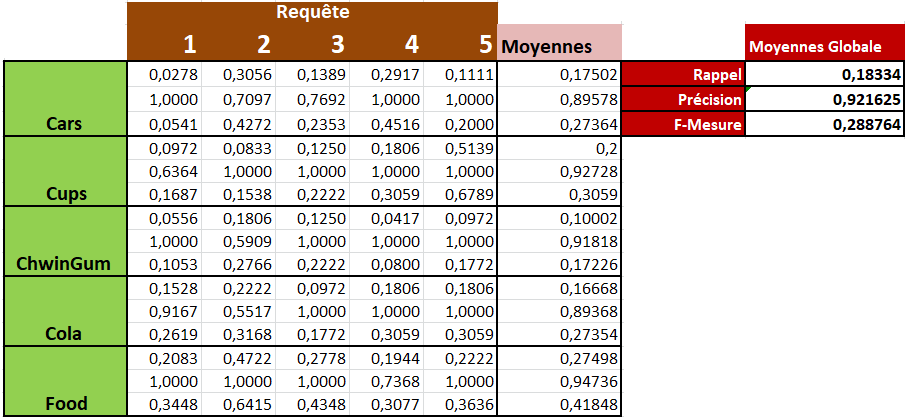
\includegraphics[width=.7\textwidth]{colShpPert} 
	\caption{Pertinence des moments de couleur combiné avec les moments de Zernike.}
\end{figure}
Les résultats donner dans la figure 4.31 ne présent pas une précision acceptable par rapport à celui donner dans la figure 4.24. Alors, nous avons changer les poids dans le but de l'améliorer comme suite:
\begin{figure}[H]
	\centering
	\includegraphics[width=.5\textwidth]{ColTxtrOptions}
	\caption{Options des moments de couleur combiné avec les filtres de Gabor (Deuxième expérience):
		20\% Couleur avec 80\% Texture.}
\end{figure}
On obtient:
\begin{figure}[H]
	\centering
	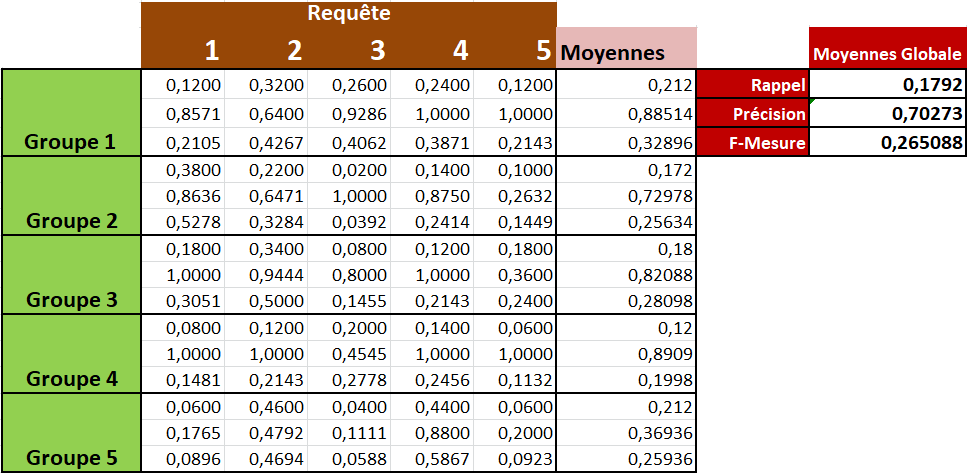
\includegraphics[width=.7\textwidth]{colTxtrPer2} 
	\caption{Pertinence des moments de couleur combiné avec les filtres de Gabor (Deuxième expérience).}
\end{figure}

En générale, on remarque que la combinaison des descripteurs améliore la précisions des résultats obtenus:
\begin{itemize}
	\item Pour la couleur et la texture: comme le montre le figures 4.34, on obtient une précision de 70\% contre  75\% (Figure 4.26) avec la texture seul (le choix des poids compte dans la qualité ici).
	\item Pour la couleur et la forme: comme le montre les figures 4.32, on obtient une précision de 92\% contre  55\% (Figure 4.29) avec la forme seul.
\end{itemize}
\section{Problèmes rencontrés}
\begin{itemize}
	\item La première problématique qui s’est imposée durant la réalisation du notre
	application est le choix des descripteurs discriminants d’image pour s’assurer de
	l’obtention des meilleurs résultats et pour une évaluation significative.
	\item Aussi le choix du modèle de couleur et la mesure de distance à utiliser.
	
	\item Et aussi les extensions des images. Dans un premier lieu nous avons travaillé
	qu’avec les images .jpg après, nous avons pu utiliser des images .png après une
	petite adaptation de code (il est possible d'ajouter d'autres format en modifiant une seul ligne de code).
	
	\item Dans la phase d'indexation de quelques descripteurs à savoir les filtres de Gabor, l'opération prend des dizaines de minutes, une qui nous a compliqué les testes d'avancement.
	\item Pour les descripteurs de forme nous avons hésiter avec la méthode de segmentation à utiliser et nous avons adobter un simple seuillage (thresholding) pour transformer les images en noir et blanc.
	\item ...etc.
\end{itemize}
\section{Perspectives}
Comme perspectives, Nous proposons :
\begin{itemize}
	\item D’utiliser les descripteurs de l'apprentissage automatique (Machine Learning).
	
	\item De Travailler avec tous les format des images existant.
	\item D’essayer autres techniques de mesures de similarité entre les descripteurs
	d’images.
    \item Tester notre application avec d’autres bases de données.
\end{itemize}
\section{Conclusion}
Au cours de ce dernier chapitre, nous avons présenté notre système de recherche d’images par le contenu où nous avons essayé d’utiliser les descripteurs connues et les mesures de similarité les plus recommandés dans la littérature. Les tests ont été effectués avec des bases d’images universellement connues. La comparaison de nos résultats avec ceux de la littérature permet de valider notre travail.